\subsection{17. Undirected Graphs and Conditional Independence}\label{undirected-graphs-and-conditional-independence}

\(k\) binary variables \(Y_1, \dots, Y_k\) correspond to a multinomial
with \(N = 2^k\) categories. Even for moderately large \(k\), \(2^k\)
will be huge. It can be shown in this case that the MLE is a poor
estimator, because the data are \textbf{sparse}.

Graphical models often require fewer parameters and may lead to
estimators with smaller risk. There are two main types of graphical
models: undirected and directed. Here we introduce undirected graphs.

\subsubsection{17.1 Conditional Independence}\label{conditional-independence}

Let \(X\), \(Y\), \(Z\) be discrete random variables. We say that \(X\)
and \(Y\) are \textbf{conditionally independent given \(Z\)}, written
\(X \text{⫫} Y \;|\; Z\), if

\[ \mathbb{P}(X = x, Y = y | Z = z) = \mathbb{P}(X = x | Z = z) \mathbb{P}(Y = y | Z = z)\]

for all \(x\), \(y\), \(z\). If \(X\), \(Y\), \(Z\) are continuous
random variables, we say that \(X\) and \(Y\) are conditionally
independent given \(Z\) if

\[ f_{X, Y | Z}(x, y | z) = f_{X | Z}(x | z) f_{Y | Z}(y | z) \]

for all \(x\), \(y\), \(z\).

Intuitively, this means that once you know \(Z\), \(Y\) provides no
extra information about \(X\).

\textbf{Theorem 17.2}. The following implications hold:

\[
\begin{align}
X \text{ ⫫ } Y \;|\; Z & \Longrightarrow Y \text{ ⫫ } X \;|\; Z \\
X \text{ ⫫ } Y \;|\; Z \; \text{and} \; U = h(X) & \Longrightarrow U \text{ ⫫ } Y \;|\; Z \\
X \text{ ⫫ } Y \;|\; Z \; \text{and} \; U = h(X) & \Longrightarrow X \text{ ⫫ } Y \;|\; (Z, U)  \\
X \text{ ⫫ } Y \;|\; Z \; \text{and} \; X \text{ ⫫ } W \;|\; (Y, Z) & \Longrightarrow X \text{ ⫫ } (W, Y) \;|\; Z \\
X \text{ ⫫ } Y \;|\; Z \; \text{and} \; X \text{ ⫫ } Z \;|\; Y \; & \Longrightarrow Y \text{ ⫫ } (Y, Z)
\end{align}
\]

The last property requires the assumption that all events have positive
probability; the first four do not.

\subsubsection{17.2 Undirected Graphs}\label{undirected-graphs}

An \textbf{undirected graph} \(\mathcal{G} = (V, E)\) has a finite set
\(V\) of \textbf{vertices} (or \textbf{nodes}) and a set \(E\) of
\textbf{edges} (or \textbf{arcs}) consisting of pairs of vertices. The
vertices correspond to random variables \(X, Y, Z, \dots\) and the edges
are written as unordered pairs. For example, \((X, Y) \in E\) means that
\(X\) and \(Y\) are joined by an edge.

\begin{python}
from graphviz import Graph

g = Graph()

g.edge('Y', 'X')
g.edge('Y', 'Z')

g
\end{python}

\begin{figure}[H]
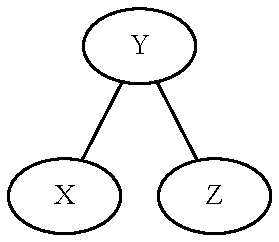
\includegraphics[width=0.9\linewidth,height=0.2\textheight,keepaspectratio]{Figure-17-01}
\end{figure}

\emph{A graph with vertices \(V = \{X, Y, Z\}\). The edge set is
\(E = \{(X, Y), (Y, Z)\}\).}

Two vertices are \textbf{adjacent}, written \(X \sim Y\), if there is an
edge between them. A sequence \(X_0, \dots, X_n\) is called a
\textbf{path} if \(X_{i-1} \sim X_i\) for each \(i\). A graph is
\textbf{complete} if there is an edge between every pair of vertices. A
subset \(U \subset V\) of vertices together with their edges is called a
\textbf{subgraph}.

If \(A\), \(B\) and \(C\) are three distinct subsets in \(V\), we say
that \textbf{\(C\) separates \(A\) and \(B\)} if every path from a
variable in \(A\) to a variable in \(B\) intersects a variable in \(C\).

\begin{python}
from graphviz import Graph

g = Graph()

g.edge('W', 'X')
g.edge('W', 'Y')
g.edge('X', 'Z')
g.edge('X', 'Y')

g
\end{python}

\begin{figure}[H]
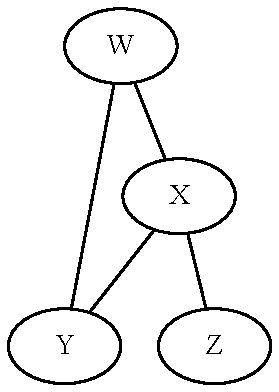
\includegraphics[width=0.9\linewidth,height=0.2\textheight,keepaspectratio]{Figure-17-02}
\end{figure}

\emph{\(\{Y, W\}\) and \(\{Z\}\) are separated by \(\{X\}\). Also, \(W\)
and \(Z\) are separated by \(\{X, Y\}\).}

\subsubsection{17.3 Probability and Graphs}\label{probability-and-graphs}

Let \(V\) be a set of random variables with distribution \(\mathbb{P}\).
Construct a graph with one vertex for each random variable in \(V\).
Suppose we omit the edge between a pair of variables if they are
independent given the rest of the variables:

\[ \text{no edge between } X \text{ and } Y \Leftrightarrow X \text{⫫} Y \;|\; \text{rest} \]

where ``rest'' refers to all the other variables besides \(X\) and
\(Y\). This type of graph is called a \textbf{pairwise Markov graph}.

The graph encodes a set of pairwise conditional independence relations.
These relations imply other conditional independence relations.
Fortunately we can read these other conditional independence relations
from the graph as well, as is explained in the next theorem.

\textbf{Theorem 17.3}. Let \(\mathcal{G} = (V, E)\) be a pairwise Markov
graph for a distribution \(\mathbb{P}\). Let \(A\), \(B\), and \(C\) be
distinct subsets of \(V\) such that \(C\) separates \(A\) and \(B\).
Then \(A \text{ ⫫ } B \;|\; C\).

Remark: if \(A\) and \(B\) are not connected, we can regard them as
separated by the empty set. Then it follows from the theorem that
\(A \text{ ⫫ } B\).

The independence property in Theorem 17.3 is called the \textbf{global
Markov property}. We thus see that the pairwise and global Markov
properties are equivalent.

More precisely: given a graph \(\mathcal{G}\),

\begin{itemize}[tightlist]
\item
  Let \(M_\text{pair}(\mathcal{G})\) be the set of distributions that
  satisfy the pairwise Markov property; thus
  \(\mathbb{P} \in M_\text{pair}(\mathcal{G})\) if, under
  \(\mathbb{P}\), \(X \text{⫫} Y \;|\; \text{rest}\) if and only if
  there is no edge between \(X\) and \(Y\).
\item
  Let \(M_\text{global}(\mathcal{G})\) be the set of distributions that
  satisfy the global Markov property; thus
  \(\mathbb{P} \in M_\text{global}(\mathcal{G})\) if, under
  \(\mathbb{P}\), \(A \text{⫫} B \;|\; C\) if and only if \(C\)
  separates \(A\) and \(B\).
\end{itemize}

\textbf{Theorem 17.5}. Let \(\mathcal{G}\) be a graph. Then
\(M_\text{pair}(\mathcal{G}) = M_\text{global}(\mathcal{G})\).

\begin{python}
from graphviz import Graph

g = Graph()

g.edge('X', 'Y')
g.edge('Y', 'Z')
g.edge('Z', 'X')

g
\end{python}
 
\begin{figure}[H]
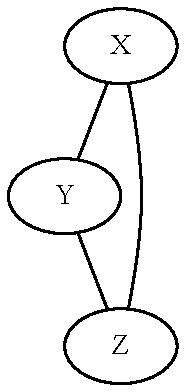
\includegraphics[width=0.9\linewidth,height=0.2\textheight,keepaspectratio]{Figure-17-03}
\end{figure}

\emph{No implied independence relations}

\begin{python}
from graphviz import Graph

g = Graph()

g.edge('X', 'Y')
g.edge('Y', 'Z')
g.edge('Z', 'W')
g.edge('W', 'X')

g
\end{python}
 
\begin{figure}[H]
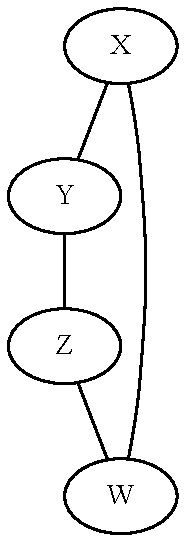
\includegraphics[width=0.9\linewidth,height=0.2\textheight,keepaspectratio]{Figure-17-04}
\end{figure}

\emph{\(X \text{ ⫫ } Z \;|\; \{Y, W\}\) and
\(Y \text{ ⫫ } W \;|\; \{X, Z\}\)}

\begin{python}
from graphviz import Graph

g = Graph()

g.edge('X', 'Y')
g.edge('Y', 'Z')
g.edge('Z', 'W')

g
\end{python}
 
\begin{figure}[H]
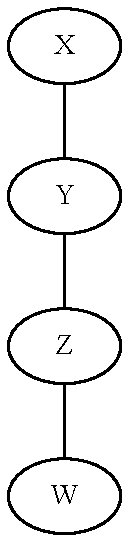
\includegraphics[width=0.9\linewidth,height=0.2\textheight,keepaspectratio]{Figure-17-05}
\end{figure}

\emph{\(X \text{ ⫫ } Z \;|\; Y\) and \(Y \text{ ⫫ } W \;|\; Z\)}

\begin{python}
from graphviz import Graph

g = Graph()

g.edge('Y', 'Z')
g.node('X')

g
\end{python}

 
\begin{figure}[H]
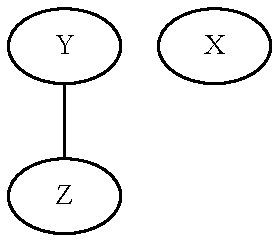
\includegraphics[width=0.9\linewidth,height=0.2\textheight,keepaspectratio]{Figure-17-06}
\end{figure}

\emph{\(X \text{ ⫫ } Y\), \(X \text{ ⫫ } Z\) and
\(X \text{ ⫫ } (Y, Z)\)}

\begin{python}
from graphviz import Graph

g = Graph()

g.edge('Y', 'W')
g.edge('W', 'Z')
g.edge('Z', 'Y')
g.edge('X', 'Y')

g
\end{python}

 
\begin{figure}[H]
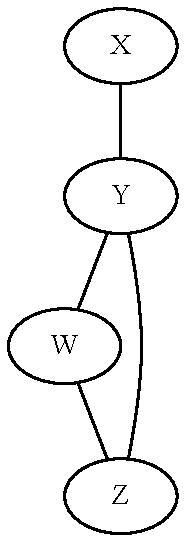
\includegraphics[width=0.9\linewidth,height=0.2\textheight,keepaspectratio]{Figure-17-07}
\end{figure}

\emph{\(X \text{ ⫫ } W | (Y, Z)\) and \(X \text{ ⫫ } Z | Y\)}

\subsubsection{17.4 Fitting Graphs to Data}\label{fitting-graphs-to-data}

Given a dataset, how do we find a graphical model that fits the data?
Some authors have devoted whole books to this subject. We will only
treat the discrete case and we will consider a method based on
\textbf{log-linear models} which are the subject of the next chapter.

\subsubsection{17.6 Exercises}\label{exercises}

\textbf{Exercise 17.6.1}. Consider random variables \((X_1, X_2, X_3)\).
In each of the following cases, draw a graph that has the given
independence relations.

\textbf{(i)} \(X_1 \text{ ⫫ } X_3 | X_2\)

\textbf{(ii)} \(X_1 \text{ ⫫ } X_2 | X_3\) and
\(X_1 \text{ ⫫ } X_3 | X_2\)

\textbf{(iii)} \(X_1 \text{ ⫫ } X_2 | X_3\) and
\(X_1 \text{ ⫫ } X_3 | X_2\) and \(X_2 \text{ ⫫ } X_3 | X_1\)

\textbf{Solution}

\textbf{(i)} \(X_1 \text{ ⫫ } X_3 | X_2\)

\begin{python}
from graphviz import Graph

g = Graph()

g.edge('X1', 'X2')
g.edge('X2', 'X3')

g
\end{python}

\begin{figure}[H]
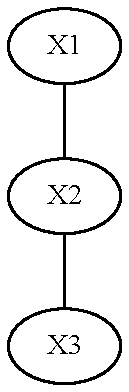
\includegraphics[width=0.9\linewidth,height=0.2\textheight,keepaspectratio]{Figure-17-08}
\end{figure}

\textbf{(ii)} \(X_1 \text{ ⫫ } X_2 | X_3\) and
\(X_1 \text{ ⫫ } X_3 | X_2\)

\begin{python}
from graphviz import Graph

g = Graph()

g.node('X1')
g.edge('X2', 'X3')

g
\end{python}
 
\begin{figure}[H]
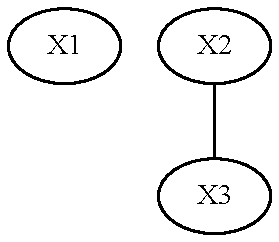
\includegraphics[width=0.9\linewidth,height=0.2\textheight,keepaspectratio]{Figure-17-09}
\end{figure}

\textbf{(iii)} \(X_1 \text{ ⫫ } X_2 | X_3\) and
\(X_1 \text{ ⫫ } X_3 | X_2\) and \(X_2 \text{ ⫫ } X_3 | X_1\)

\begin{python}
from graphviz import Graph

g = Graph()

g.node('X1')
g.node('X2')
g.node('X3')

g
\end{python}
 
\begin{figure}[H]
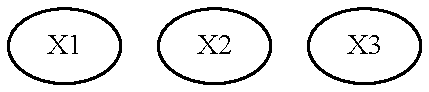
\includegraphics[width=0.9\linewidth,height=0.2\textheight,keepaspectratio]{Figure-17-10}
\end{figure}

\textbf{Exercise 17.6.2}. Consider random variables
\((X_1, X_2, X_3, X_4)\). In each of the following cases, draw a graph
that has the given independence relations.

\textbf{(a)} \$X\_1 \text{ ⫫ } X\_3 \textbar{} X\_2, X\_4 \$ and \$X\_1
\text{ ⫫ } X\_4 \textbar{} X\_2, X\_3 \$ and \$X\_2 \text{ ⫫ } X\_4
\textbar{} X\_1, X\_3 \$

\textbf{(b)} \$X\_1 \text{ ⫫ } X\_2 \textbar{} X\_3, X\_4 \$ and \$X\_1
\text{ ⫫ } X\_3 \textbar{} X\_2, X\_4 \$ and \$X\_2 \text{ ⫫ } X\_3
\textbar{} X\_1, X\_4 \$

\textbf{(c)} \$X\_1 \text{ ⫫ } X\_3 \textbar{} X\_2, X\_4 \$ and \$X\_2
\text{ ⫫ } X\_4 \textbar{} X\_1, X\_3 \$

\textbf{Solution}

\textbf{(a)} \$X\_1 \text{ ⫫ } X\_3 \textbar{} X\_2, X\_4 \$ and \$X\_1
\text{ ⫫ } X\_4 \textbar{} X\_2, X\_3 \$ and \$X\_2 \text{ ⫫ } X\_4
\textbar{} X\_1, X\_3 \$

\begin{python}
from graphviz import Graph

g = Graph()

g.edge('X1', 'X2')
g.edge('X2', 'X3')
g.edge('X3', 'X4')

g
\end{python}

\begin{figure}[H]
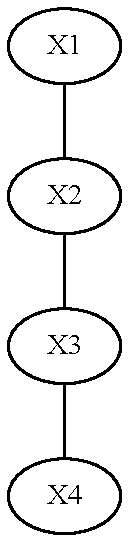
\includegraphics[width=0.9\linewidth,height=0.2\textheight,keepaspectratio]{Figure-17-11}
\end{figure}

\textbf{(b)} \$X\_1 \text{ ⫫ } X\_2 \textbar{} X\_3, X\_4 \$ and \$X\_1
\text{ ⫫ } X\_3 \textbar{} X\_2, X\_4 \$ and \$X\_2 \text{ ⫫ } X\_3
\textbar{} X\_1, X\_4 \$

\begin{python}
from graphviz import Graph

g = Graph()

g.edge('X1', 'X4')
g.edge('X2', 'X4')
g.edge('X3', 'X4')

g
\end{python}
 
\begin{figure}[H]
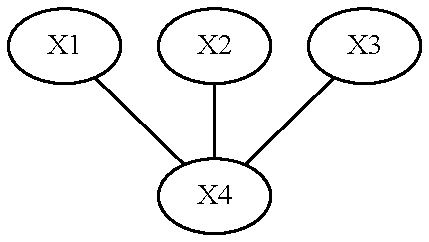
\includegraphics[width=0.9\linewidth,height=0.2\textheight,keepaspectratio]{Figure-17-12}
\end{figure}


\textbf{(c)} \$X\_1 \text{ ⫫ } X\_3 \textbar{} X\_2, X\_4 \$ and \$X\_2
\text{ ⫫ } X\_4 \textbar{} X\_1, X\_3 \$

\begin{python}
from graphviz import Graph

g = Graph()

g.edge('X1', 'X2')
g.edge('X2', 'X3')
g.edge('X3', 'X4')
g.edge('X1', 'X4')

g
\end{python}

\begin{figure}[H]
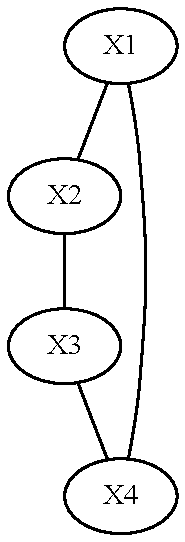
\includegraphics[width=0.9\linewidth,height=0.2\textheight,keepaspectratio]{Figure-17-13}
\end{figure}

\textbf{Exercise 17.6.3}. A conditional independence between a pair of
variables is \textbf{minimal} if it is not possible to use the
Separation Theorem to eliminate any variable from the conditioning set,
i.e.~from the right side of the bar (Whittaker 1990). Write down the
minimal conditioning independences from the given figures.

\textbf{(a)}

\begin{python}
from graphviz import Graph

g = Graph()

g.edge('X1', 'X2')
g.edge('X2', 'X3')
g.edge('X2', 'X4')

g
\end{python}

\begin{figure}[H]
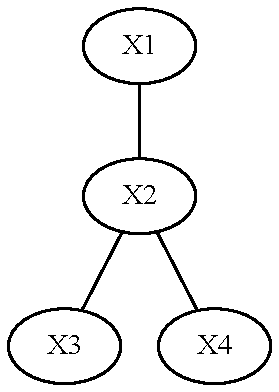
\includegraphics[width=0.9\linewidth,height=0.2\textheight,keepaspectratio]{Figure-17-14}
\end{figure}

\textbf{(b)}

\begin{python}
from graphviz import Graph

g = Graph()

g.edge('X1', 'X2')
g.edge('X2', 'X3')
g.edge('X3', 'X4')

g
\end{python}
 
\begin{figure}[H]
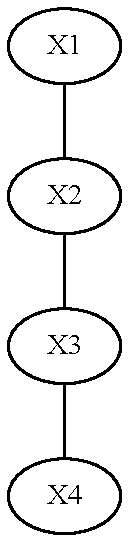
\includegraphics[width=0.9\linewidth,height=0.2\textheight,keepaspectratio]{Figure-17-15}
\end{figure}

\textbf{(c)}

\begin{python}
from graphviz import Graph

g = Graph()

g.edge('X1', 'X2')
g.edge('X2', 'X3')
g.edge('X3', 'X4')
g.edge('X4', 'X1')

g
\end{python}

\begin{figure}[H]
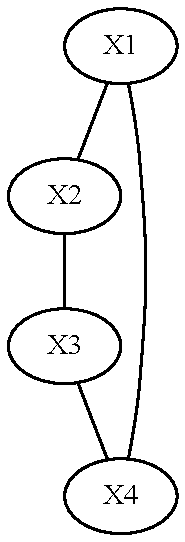
\includegraphics[width=0.9\linewidth,height=0.2\textheight,keepaspectratio]{Figure-17-16}
\end{figure}

\textbf{(d)}

\begin{python}
from graphviz import Graph

g = Graph()

g.edge('X1', 'X2')
g.edge('X2', 'X3')
g.edge('X3', 'X1')

g.edge('X2', 'X4')
g.edge('X4', 'X5')
g.edge('X5', 'X2')

g.edge('X3', 'X5')
g.edge('X5', 'X6')
g.edge('X6', 'X3')

g
\end{python}

\begin{figure}[H]
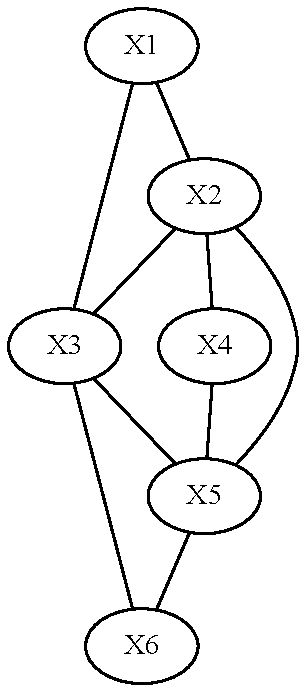
\includegraphics[width=0.9\linewidth,height=0.2\textheight,keepaspectratio]{Figure-17-17}
\end{figure}

\textbf{Solution}

\textbf{(a)}

\begin{itemize}[tightlist]
\item
  \$X\_1 \text{ ⫫ } X\_3 \textbar{} X\_2 \$
\item
  \$X\_1 \text{ ⫫ } X\_4 \textbar{} X\_2 \$
\item
  \$X\_3 \text{ ⫫ } X\_4 \textbar{} X\_2 \$
\end{itemize}

\textbf{(b)}

\begin{itemize}[tightlist]
\item
  \$X\_1 \text{ ⫫ } X\_3 \textbar{} X\_2 \$
\item
  \$X\_2 \text{ ⫫ } X\_4 \textbar{} X\_2 \$
\item
  \$X\_1 \text{ ⫫ } X\_4 \textbar{} X\_2 \$ (or \$X\_1 \text{ ⫫ } X\_4
  \textbar{} X\_3 \$)
\end{itemize}

\textbf{(c)}

\begin{itemize}[tightlist]
\item
  \$X\_1 \text{ ⫫ } X\_3 \textbar{} X\_2, X\_4 \$
\item
  \$X\_2 \text{ ⫫ } X\_4 \textbar{} X\_1, X\_3 \$
\end{itemize}

\textbf{(d)}

\begin{itemize}[tightlist]
\item
  \$X\_1 \text{ ⫫ } X\_4 \textbar{} X\_2, X\_3 \$ ( or \$X\_1 \text{ ⫫ }
  X\_4 \textbar{} X\_2, X\_5 \$ )
\item
  \$X\_1 \text{ ⫫ } X\_5 \textbar{} X\_2, X\_3 \$
\item
  \$X\_1 \text{ ⫫ } X\_6 \textbar{} X\_2, X\_3 \$ ( or \$X\_1 \text{ ⫫ }
  X\_6 \textbar{} X\_2, X\_5 \$ )
\item
  \$X\_2 \text{ ⫫ } X\_6 \textbar{} X\_3, X\_5 \$
\item
  \$X\_3 \text{ ⫫ } X\_4 \textbar{} X\_2, X\_5 \$
\item
  \$X\_4 \text{ ⫫ } X\_6 \textbar{} X\_2, X\_5 \$ ( or \$X\_4 \text{ ⫫ }
  X\_6 \textbar{} X\_3, X\_5 \$ )
\end{itemize}

\textbf{Exercise 17.6.4}. Here are the breast cancer data on diagnosic
center (\(X_1\)), nuclear grade (\(X_2\)) and survival (\(X_3\)):

\[
\begin{array}{cccccc}
    & X_2 & \text{malignant} & \text{malignant} & \text{benign} & \text{benign}   \\
    & X_3 & \text{died}      & \text{survived}  & \text{died}   & \text{survived} \\
\hline
X_1 & \text{Boston}    & 35 & 59 & 47 & 112 \\
    & \text{Glamorgan} & 42 & 77 & 26 & 76 \\
\hline
\end{array}
\]

\textbf{(a)} Treat this as a multinomial and find the maximum likelihood
estimator.

\textbf{(b)} If someone has a tumour classified as benign at the
Glamorgan clinic, what is the estimated probability that they will die?
Find the standard error for this estimate.

\textbf{(c)} Test the following hypothesis:

\[
\begin{align}
X_1 \text{ ⫫ } X_2 |  X_3 \quad &\text{versus} \quad \text{not} (X_1 \text{ ⫫ } X_2 |  X_3 ) \\
X_1 \text{ ⫫ } X_3 |  X_2 \quad &\text{versus} \quad \text{not} (X_1 \text{ ⫫ } X_3 |  X_2 ) \\
X_2 \text{ ⫫ } X_3 |  X_1 \quad &\text{versus} \quad \text{not} (X_2 \text{ ⫫ } X_3 |  X_1 ) \\
\end{align}
\]

Based on the results of your tests, draw and interpret the resulting
graph.

\textbf{Solution}.

\textbf{(a)}

\begin{python}
import numpy as np

X = np.array([[[35, 59], [47, 112]], [[42, 77], [26, 76]]])
\end{python}

\begin{python}
p_hat = X / X.sum()

p_hat
\end{python}

\begin{console}
array([[[0.07383966, 0.12447257],
        [0.09915612, 0.23628692]],

       [[0.08860759, 0.16244726],
        [0.05485232, 0.16033755]]])
\end{console}

\textbf{(b)} The question asks for
\(\mathbb{P}( X_3 = \text{died} | X_1 = \text{Glamorgan}, X_2 = \text{benign})\).
The MLE estimate is:

\[\hat{p} = \frac{26}{26 + 76} \approx 0.2594\]

The distribution is a binomial distribution on only \(X_3\), conditioned
on the other variables.

The variance is

\[\mathbb{V}(\hat{p}) = \frac{1}{n}\hat{p} (1 - \hat{p}) = \frac{1}{26 + 76} \frac{26}{26 + 76} \frac{76}{26 + 76}  \approx 0.001862\]

so the standard deviation of this estimate is approximately \(0.0431\).

\textbf{(c)}

We will test conditional independence \(A \text{ ⫫ } B \;|\; C\) over
discrete variables \(A\), \(B\) and \(C\) by testing independence
between \(A\) and \(B\) for each value of \(C = c\) and then selecting
the largest / worst p-value.

\begin{python}
from scipy.stats import chi2_contingency

def get_p_value(table):
    # Implement Pearson's chi squared independence test
    chi2, p, dof, expected = chi2_contingency(table)
    return p
\end{python}

\begin{python}
p_12 = max([get_p_value(X[:, :, k]) for k in range(X.shape[2])])
p_13 = max([get_p_value(X[:, k, :]) for k in range(X.shape[1])])
p_23 = max([get_p_value(X[k, :, :]) for k in range(X.shape[1])])

print("X_1 ⫫ X_2 | X_3:  %.3f" % p_12)
print("X_1 ⫫ X_3 | X_2:  %.3f" % p_13)
print("X_2 ⫫ X_3 | X_1:  %.3f" % p_23)
\end{python}

\begin{console}
X\_1 ⫫ X\_2 | X\_3:  0.030
X\_1 ⫫ X\_3 | X\_2:  0.882
X\_2 ⫫ X\_3 | X\_1:  0.262
\end{console}

At a confidence level of 5\%, we can certify the first hypothesis, but
not the other two.

The resulting graph would be:

\begin{python}
from graphviz import Graph

g = Graph()

g.edge('X1 (diagnostic center)', 'X3 (survival)')
g.edge('X3 (survival)', 'X2 (nuclear grade)')

g
\end{python}

\begin{figure}[H]
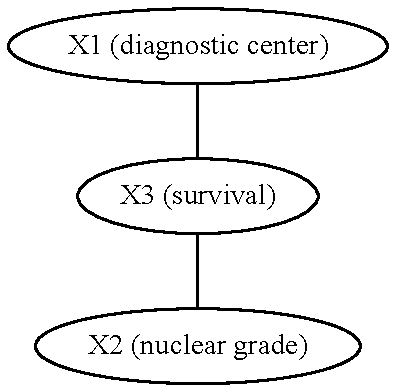
\includegraphics[width=0.9\linewidth,height=0.2\textheight,keepaspectratio]{Figure-17-18}
\end{figure}

These results can be interpreted to mean that the nuclear grade is
independent of the diagnostic center given the survival -- that is, no
diagnostic center is more optimistic or pessimistic in its
classification of tumors given their severity.
